Next a slice at $z=\SI{40}{nm}$ is compared to the original simulation by \cite{heeg} in figure \ref{slice-comparision}.

\begin{figure}[!h]
  \centering
  \begin{subfigure}{0.50\textwidth}
    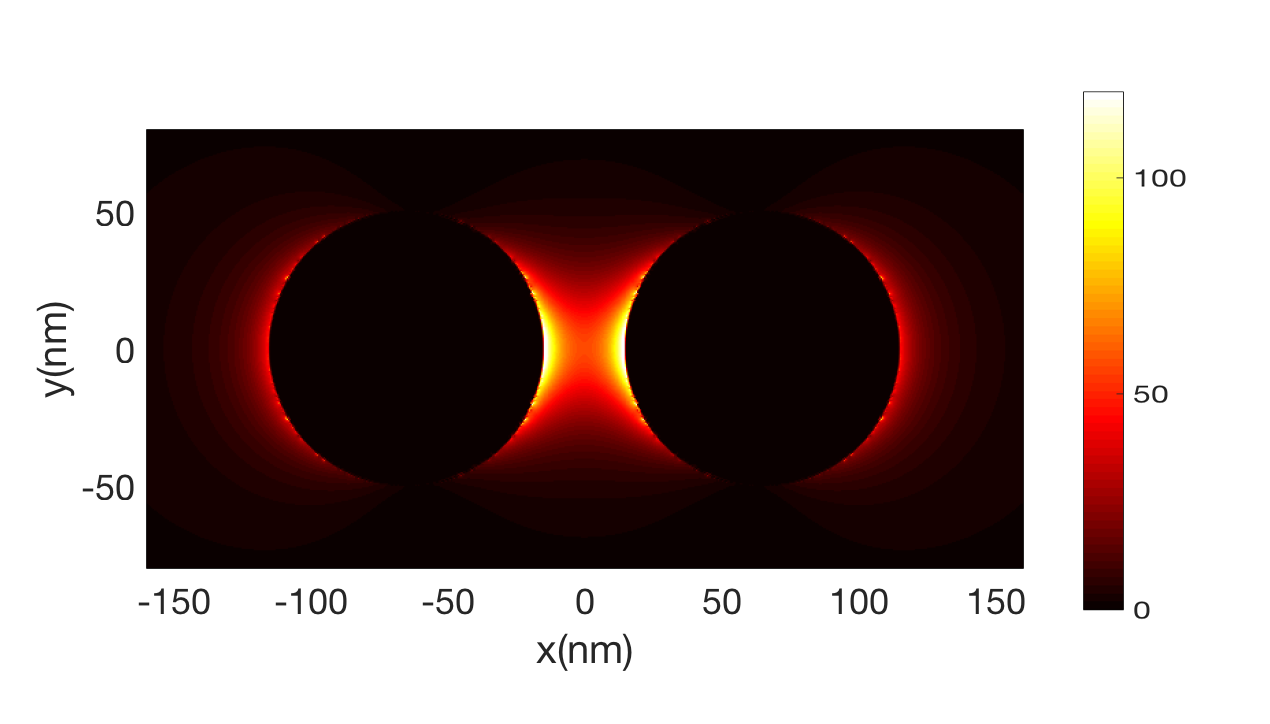
\includegraphics[width=\textwidth]{./images/40nm.png}
  \end{subfigure}
  ~
  \begin{subfigure}{0.40\textwidth}
    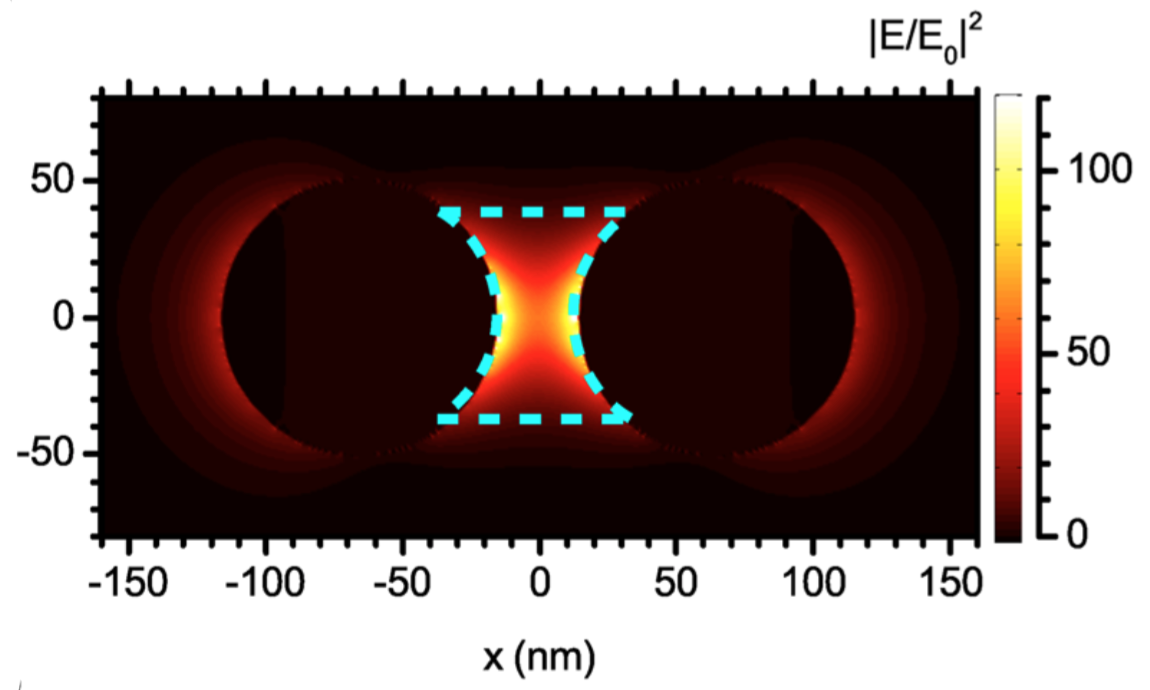
\includegraphics[width=\textwidth]{./images/local-enhancement-heeg.png}
    \label{heeg-result}
  \end{subfigure}
  \label{slice-comparision}
  \caption{\textbf{(a)} Near field enhancement $|E/E_0|^2$ in the $x,y$-plane at $z=\SI{40}{nm}$. \textbf{(b)} Original results by \cite{heeg}.}
\end{figure}

\note{compare lumerical simulation with original heeg results: simulation gives same results as original paper. same shape, same values in most areas. slight changes directly next to the nano structure.}

\begin{figure}[!h]
  \centering
  \begin{subfigure}{0.45\textwidth}
    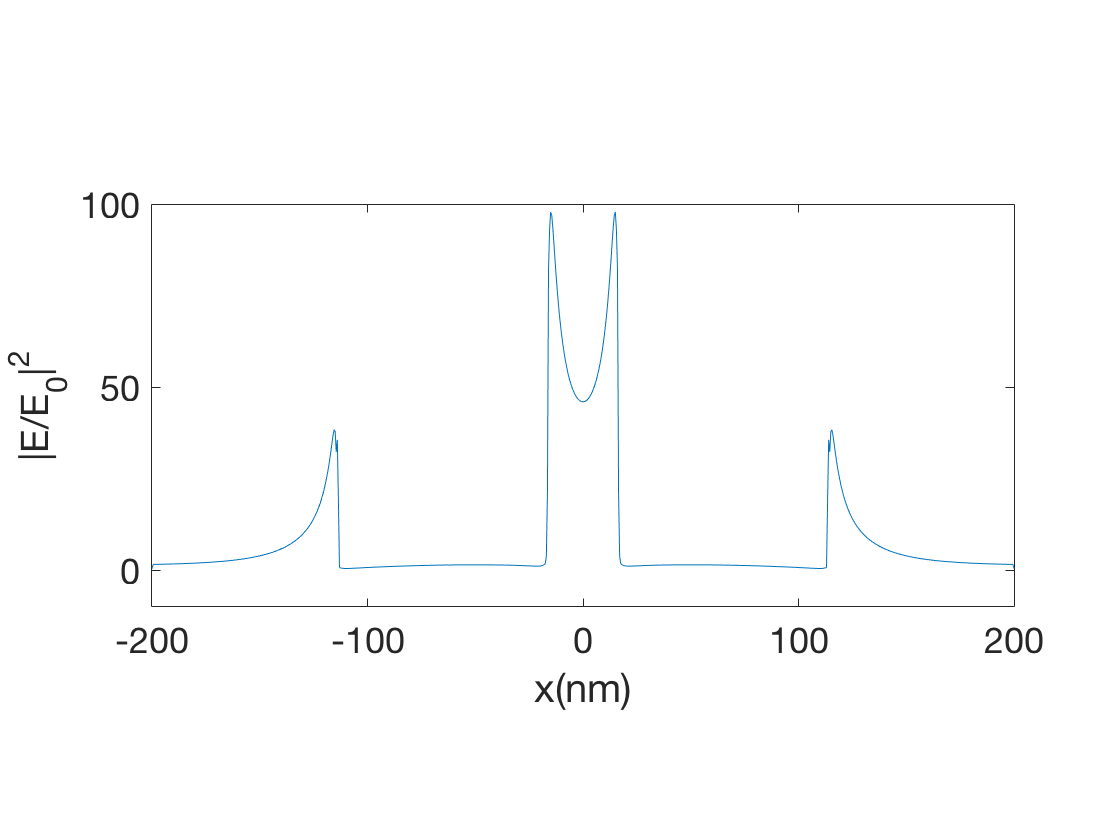
\includegraphics[width=\textwidth]{./images/40nm-y.png}
  \end{subfigure}
  ~
  \begin{subfigure}{0.45\textwidth}
    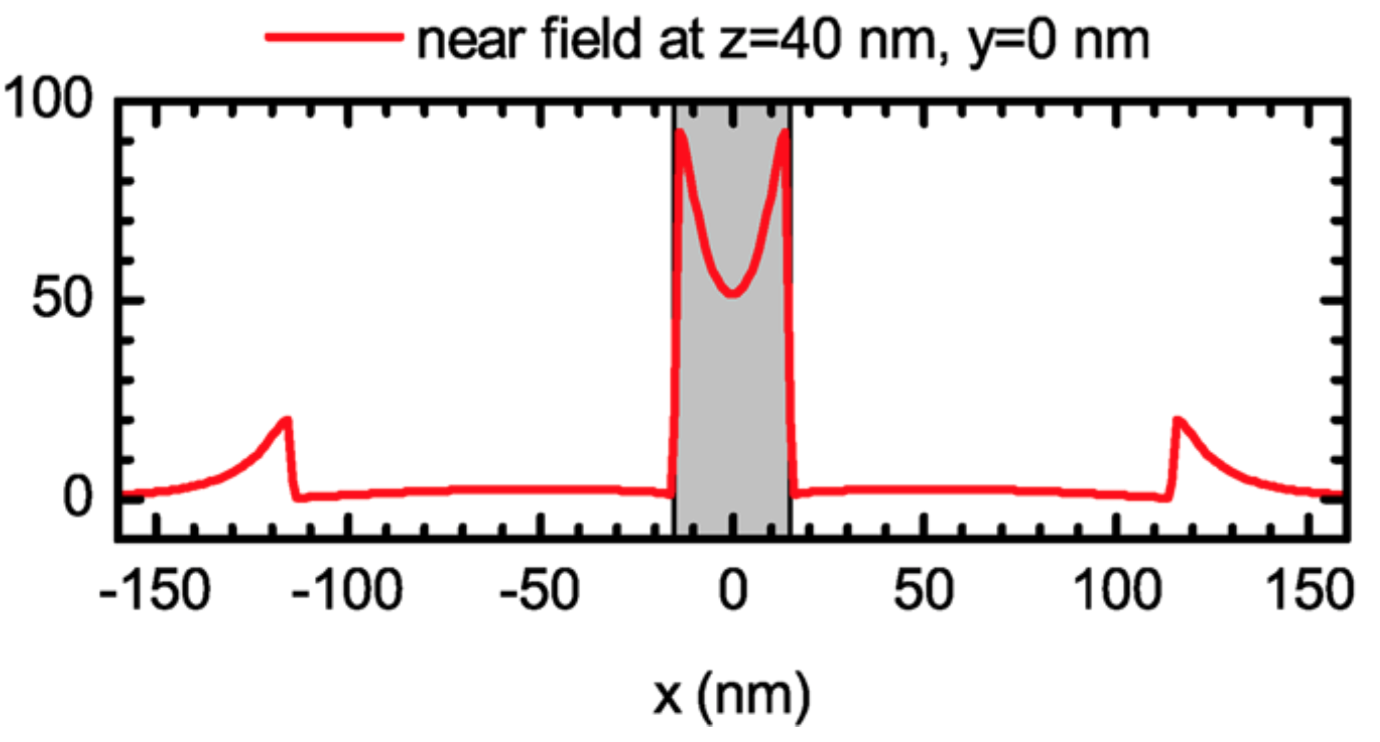
\includegraphics[width=\textwidth]{./images/heeg-y-line.png}
  \end{subfigure}
  \caption{\textbf{(a)} Near field enhancement $|E/E_0|^2$ in the $x,z$-plane at $y=0$. \textbf{(b)} Original results by \cite{heeg}.}
\end{figure}

\note{same shape of the graph in the cavity, same minimum and maximum of 100/50. higher values on the outer corners of nano structure, maybe due to corner radius. grey area contains 90\% of enhancement according to heeg.}

\newpage
\null
